

\subsection{Iteración 2}

En esta iteración se procede a la creación de los distintos escenarios y decorados para el proyecto. Para esto se puede utilizar cualquier software de modelado 3D, incluso el propio Unity. Se ha elegido utilizar Blender, una herramienta totalmente gratuita y de las más potentes del mercado.


\subsubsection{Escenario principal}

Todas las partes básicas del escenario se han creado en Blender como un único elemento formado internamente por distintas partes. Se ha comenzado creando una plataforma circular donde estará el usuario, a la cual se le ha añadido un suelo inferior también circular. Para completar la parte central de escenario (figura \ref{fig:E3_escenarioCentral}), se añaden unas gradas en la mitad posterior del círculo. Para crear las gradas se ha recurrido a la técnica de revolución de un perfil, que consiste en diseñar únicamente el perfil del objeto deseado y posteriormente hacerlo girar sobre un eje para crear un objeto en la zona que barre el perfil.

\begin{figure}
  \centering
    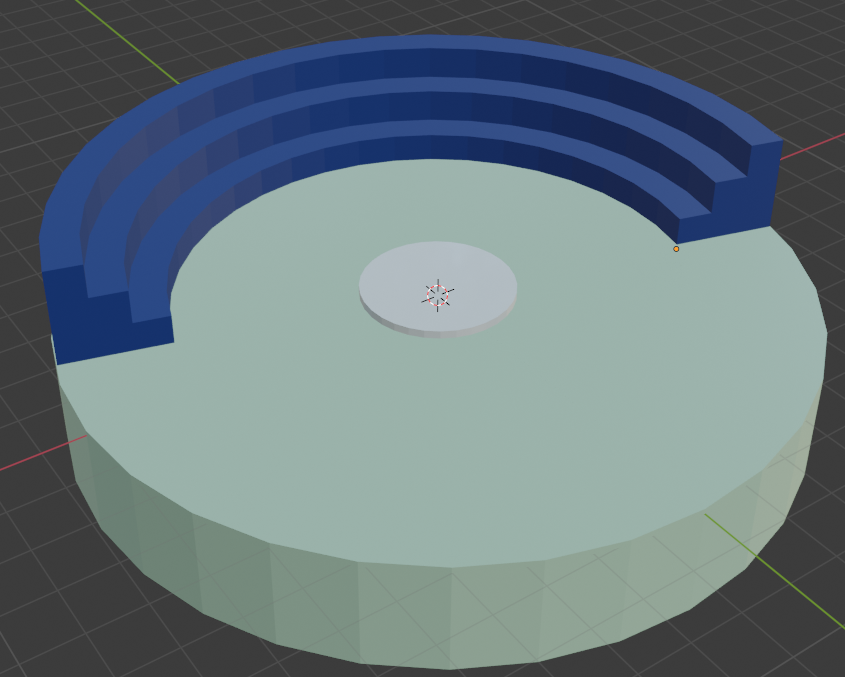
\includegraphics[width=0.5\textwidth]{04.Desarrollo/03.Entrega3/02.Iteracion3_2/00.Figuras/01.escenario_5.png}
    \caption{Parte central del escenario.}
    \label{fig:E3_escenarioCentral}
\end{figure}

Como parte del proceso continuo de mejora del proyecto, se decide que determinadas pruebas transcurran en una zona concreta del escenario con una ambientación más adecuada. Estas pruebas son las que conllevan amplios movimientos del usuario: baile, posiciones, parada y objetivos, por eso, la ambientación de esta nueva zona consistirá en colocar un escenario de baile desde el cual recibirá la prueba el jugador. Se añade también una pared para encapsular el escenario dentro del espacio virtual (figura \ref{fig:E3_escenario2}).


\begin{figure}
  \centering
    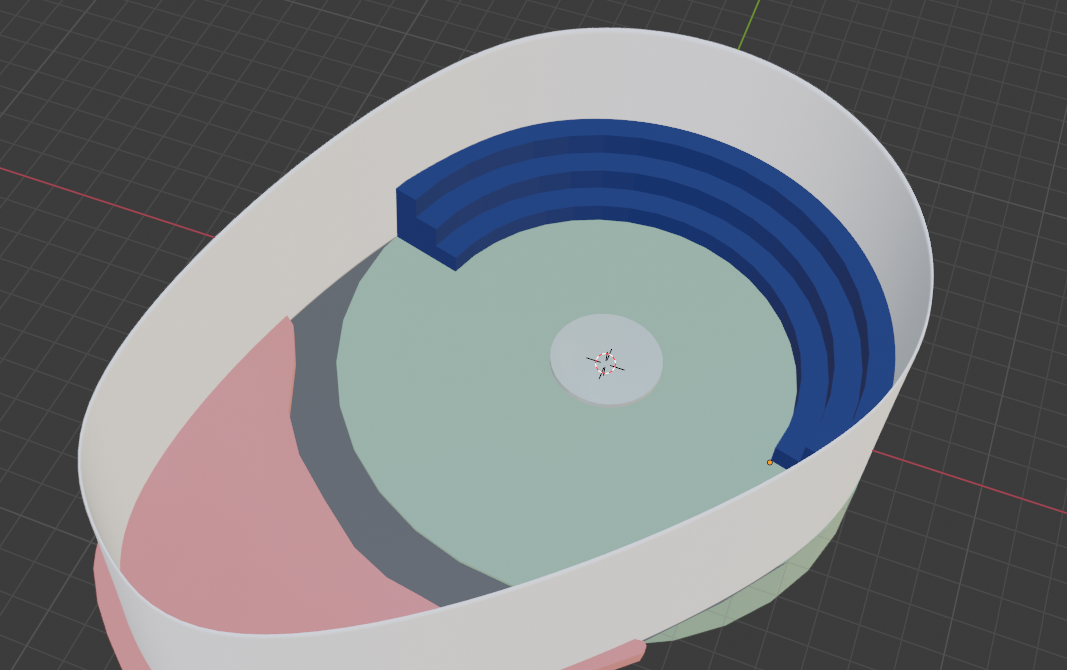
\includegraphics[width=0.5\textwidth]{04.Desarrollo/03.Entrega3/02.Iteracion3_2/00.Figuras/02.escenario_6.png}
    \caption{Plataforma principal con el escenario de baile y las paredes que rodean todo el perímetro.}
    \label{fig:E3_escenario2}
\end{figure}

En el siguiente paso en la creación de la base para el escenario de juego, se añade una pantalla para que el jugador pueda recibir información mediante texto e imágenes, un pequeño pedestal frente al escenario donde el jugador se trasladará para realizar las pruebas pertinentes, y finalmente se ha recortado un agujero en el suelo del escenario por donde bajarán y subirán los decorados de cada prueba individual. Estos cambios se pueden apreciar en la figura \ref{fig:E3_escenario3}.

\begin{figure}
  \centering
    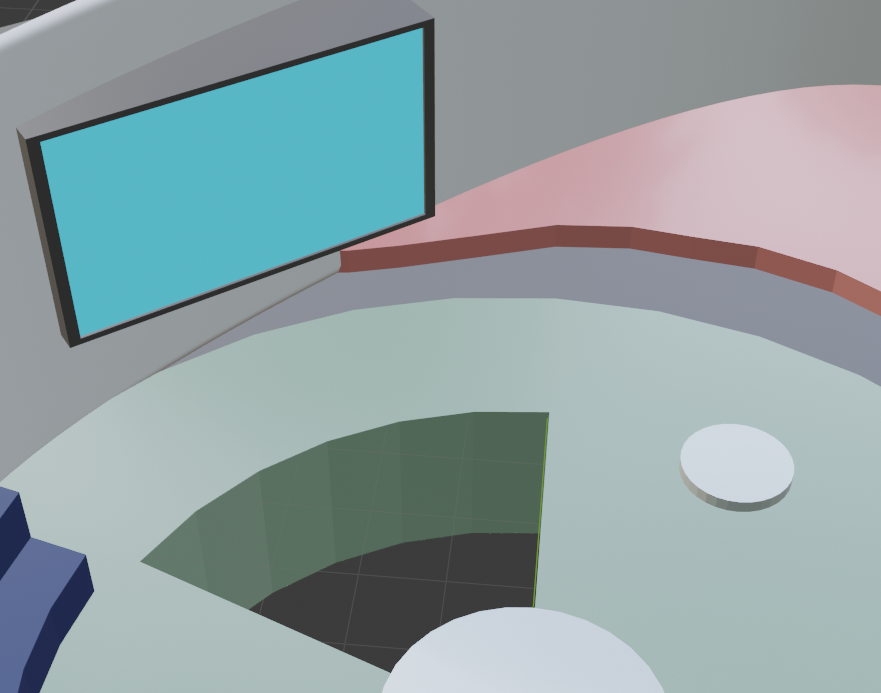
\includegraphics[width=0.5\textwidth]{04.Desarrollo/03.Entrega3/02.Iteracion3_2/00.Figuras/03.escenario_7.png}
    \caption{Detalle de la colocación de la pantalla, el pedestal secundario y el hueco del ascensor.}
    \label{fig:E3_escenario3}
\end{figure}


Finalmente se construye el ascensor que ocupará el hueco y se usará como base para el decorado de las pruebas individuales. Para ello se ha diseñado un ascensor modular que puede adaptarse a las necesidades de cada prueba, pudiendo ser utilizado en su forma básica: proporcionando únicamente un suelo (figura \ref{fig:E3_ascensorVacio}); llevando integrada una mesa en la que aparecerán objetos con los que el jugador podrá interactuar (figura \ref{fig:E3_ascensorMesa}); o con una extensión para la mesa que permite colocar mayor cantidad de objetos en ella (figura \ref{fig:E3_ascensorMesaExtendida}).


\begin{figure}
\centering
\begin{minipage}{.3\textwidth}
  \centering
  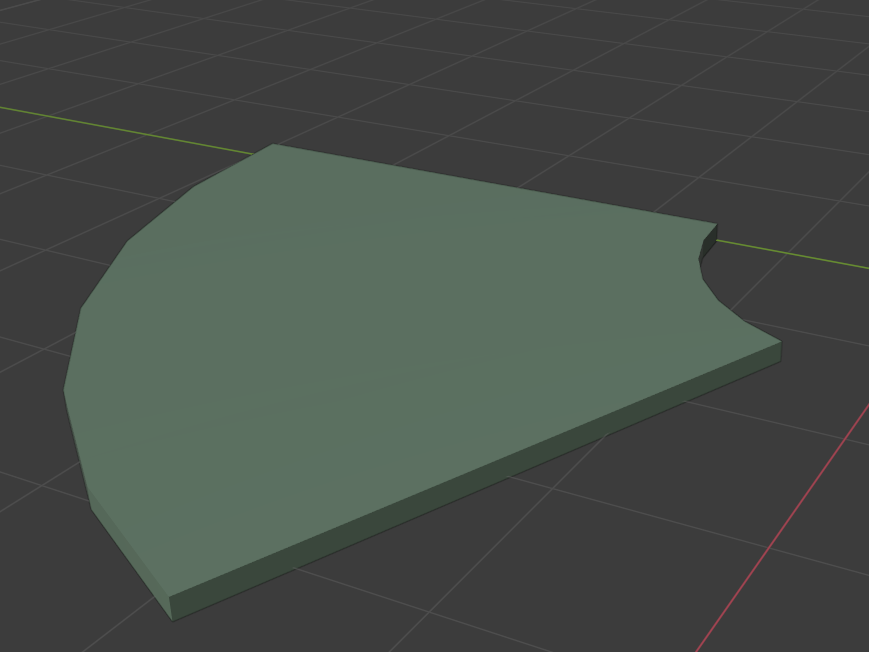
\includegraphics[width=.9\linewidth]{04.Desarrollo/03.Entrega3/02.Iteracion3_2/00.Figuras/04.ascensor_3.png}
  \captionof{figure}{Ascensor simple.}
  \label{fig:E3_ascensorVacio}
\end{minipage}%
\begin{minipage}{.3\textwidth}
  \centering
  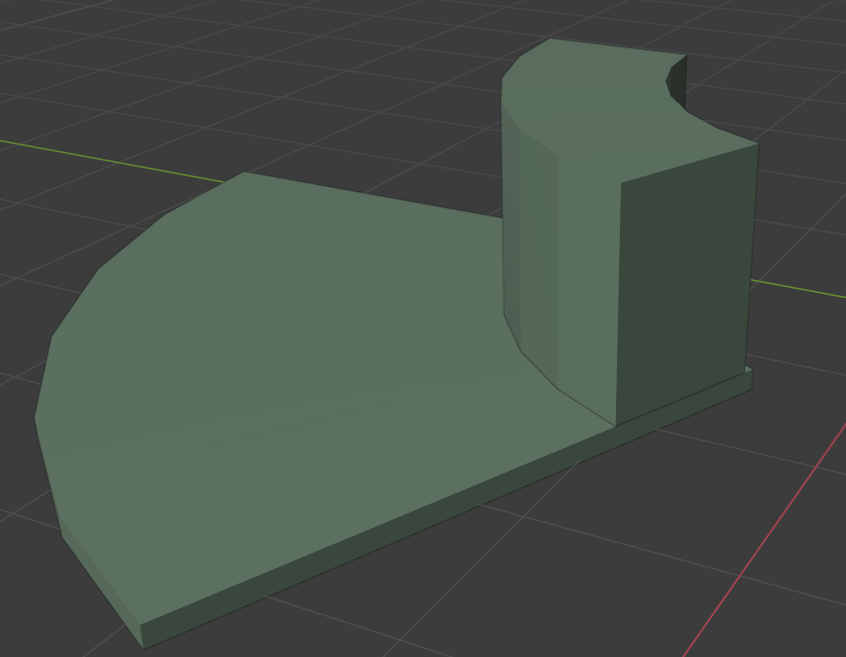
\includegraphics[width=.87\linewidth]{04.Desarrollo/03.Entrega3/02.Iteracion3_2/00.Figuras/05.ascensor_2.png}
  \captionof{figure}{Ascensor con mesa.}
  \label{fig:E3_ascensorMesa}
\end{minipage}
\begin{minipage}{.3\textwidth}
  \centering
  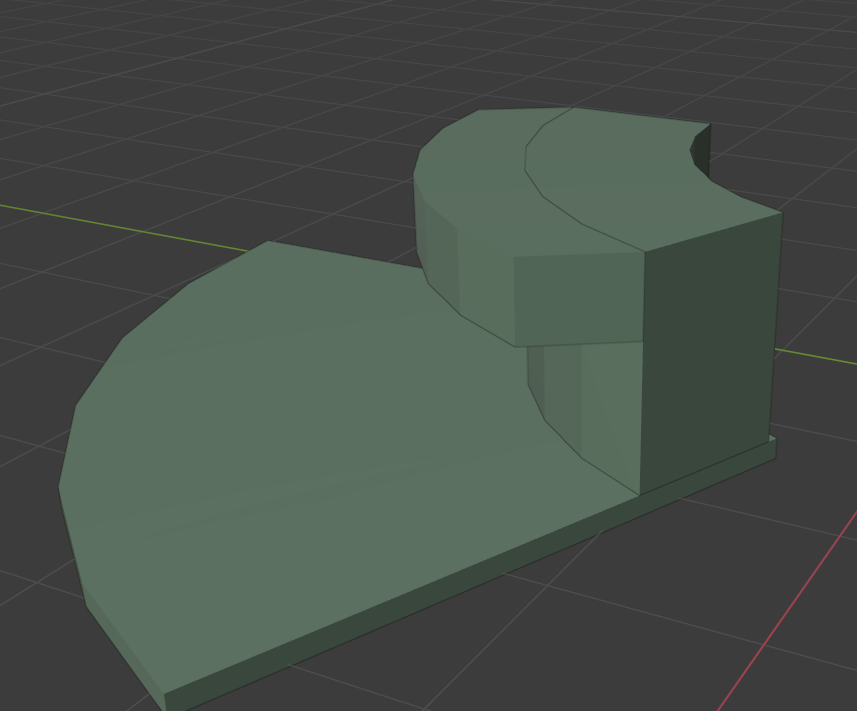
\includegraphics[width=.77\linewidth]{04.Desarrollo/03.Entrega3/02.Iteracion3_2/00.Figuras/06.ascensor_1.png}
  \captionof{figure}{Ascensor con mesa extendida.}
  \label{fig:E3_ascensorMesaExtendida}
\end{minipage}
\end{figure}





\subsubsection{Escenarios secundarios}


El decorado de los escenarios secundarios consta de una mezcla de objetos creados en Blender y una serie de objetos que ofrece Asset Store, la plataforma oficial de Unity para la distribución de contenido para ser utilizado en diversos proyectos. 

Para las pruebas de movimiento, hay que decorar el escenario de baile, para esto se han utilizado modelos de distintos instrumentos musicales (guitarra, piano, bajo y trompeta), así como un micrófono. Para dar vida a los músicos se ha utilizado un modelo de humano caricaturizado, que además se utilizará para representar todos los movimientos que el jugador necesita realizar. Por último, se han añadido unas estructuras de iluminación y varios focos en la parte superior del escenario. Véase figura \ref{fig:E3_escenarioBaile}.

\begin{figure}
  \centering
    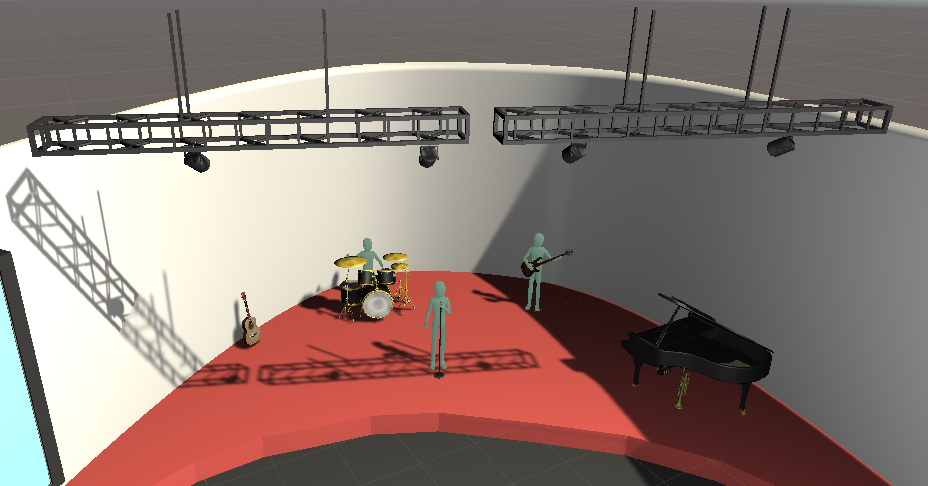
\includegraphics[width=0.5\textwidth]{04.Desarrollo/03.Entrega3/02.Iteracion3_2/00.Figuras/07.unity_1.png}
    \caption{Vista del escenario de baile completo.}
    \label{fig:E3_escenarioBaile}
\end{figure}

Además, para la prueba de objetivos se han creado dos cubos biselados en colores azul y rojo (figura \ref{fig:E3_modelosObjetivos}) que representarán los objetivos que el jugador debe golpear.

\begin{figure}
  \centering
    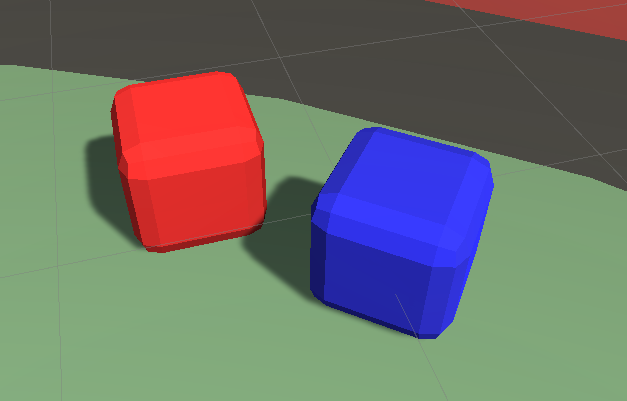
\includegraphics[width=0.5\textwidth]{04.Desarrollo/03.Entrega3/02.Iteracion3_2/00.Figuras/08.unity_5.png}
    \caption{Modelos para los objetivos que el jugador debe golpear.}
    \label{fig:E3_modelosObjetivos}
\end{figure}

El decorado para la prueba de turismo utiliza el ascensor sin mesa y adorna el espacio entre el jugador y la pantalla con objetos de temática viajera. En este caso como se ve en la figura \ref{fig:E3_escenarioTurismo}, se han colocado un globo aerostático, un avión de pasajeros despegando y en el centro un globo terráqueo.


\begin{figure}
  \centering
    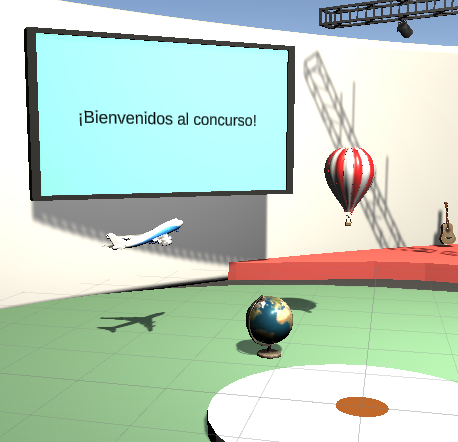
\includegraphics[width=0.5\textwidth]{04.Desarrollo/03.Entrega3/02.Iteracion3_2/00.Figuras/09.unity_2.png}
    \caption{Presentación del decorado para la prueba de turismo.}
    \label{fig:E3_escenarioTurismo}
\end{figure}


Para la prueba donde el jugador debe adivinar una canción que está sonando se ha utilizado el ascensor con mesa, en la cual se han colocado varios objetos del mundo de la música (figura \ref{fig:E3_escenarioCancion}). En el centro se han colocado unos auriculares de diadema, mientras que a cada uno de sus lados hay un dispositivo cuyo uso es reproducir música: un tocadiscos y una radio. Se han elegido objetos de estética antigua ya que resultarán más familiares al público objetivo de este proyecto, que son las personas mayores.

\begin{figure}
  \centering
    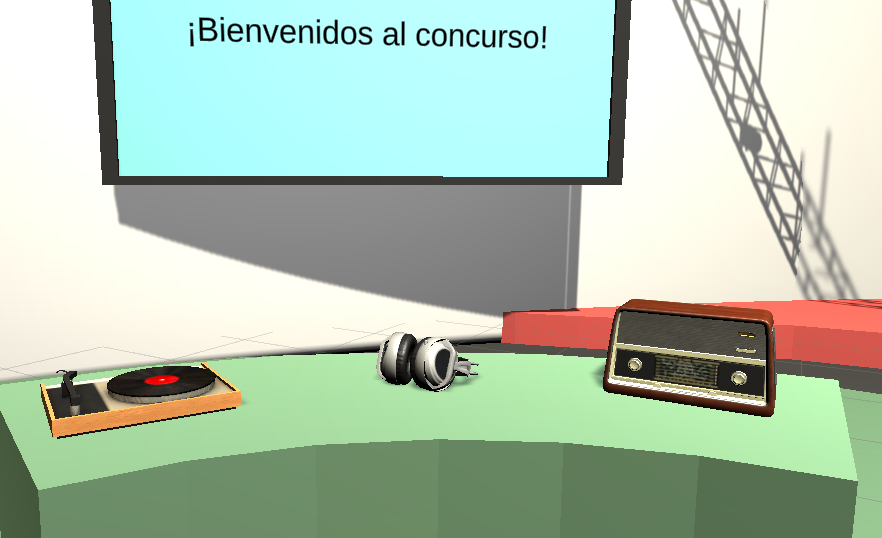
\includegraphics[width=0.5\textwidth]{04.Desarrollo/03.Entrega3/02.Iteracion3_2/00.Figuras/10.unity_3.png}
    \caption{Mesa con decorado para la prueba de adivinar la canción.}
    \label{fig:E3_escenarioCancion}
\end{figure}

El resto de las pruebas utilizan objetos virtuales para su realización, por lo que la inclusión de objetos decorativos similares podría llevar a confusión, por ejemplo, en la prueba de agrupación de objetos. Aun así, se seguirá utilizando el patrón ya marcado de utilizar los tres tipos de ascensor diseñados, pero en lugar de contener decorado, contendrán los objetos necesarios para las pruebas.

Para finalizar la decoración del escenario general y generar un ambiente más acogedor para el jugador, se han poblado las gradas con modelados caricaturizados como los músicos del escenario de baile (figura \ref{fig:E3_escenarioPublico}).


\begin{figure}
  \centering
    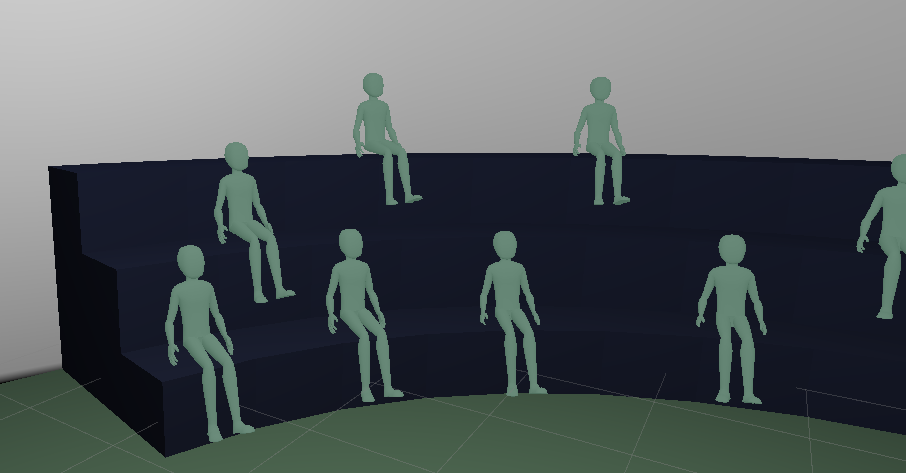
\includegraphics[width=0.5\textwidth]{04.Desarrollo/03.Entrega3/02.Iteracion3_2/00.Figuras/11.unity_4.png}
    \caption{Presentación de las figuras que actúan como público.}
    \label{fig:E3_escenarioPublico}
\end{figure}


